\chapter{Fundamentação Teórica}\label{teoria}

\section{Processos de Formação do Granizo e Eletrificação de Tempestades}\label{granizo_eletrificacao}

A \autoref{processos_crescimento} apresenta os processos primários de crescimento de hidrometeoros dentro de uma nuvem fria através da colisão entre os mesmos. O granizo é formado a partir da acreção (coleta de água superresfriada ou cristais de gelo pequenos por uma partícula de gelo maior) em gotas de chuva congeladas ou graupel, sendo o último formado a partir do processo denominado \textit{riming} (acreção de gotículas de água superresfriada em partículas de gelo em um depósito de baixa densidade) em cristais de gelo, neve ou gotas de chuva congeladas \cite{Reinking1975}. Esses processos são altamente influenciados pela quantidade e tamanho de gotas superresfriadas (ou conteúdo de água líquida) na região de fase mista da nuvem, intensidade da corrente ascendente e temperatura.

\begin{figure}[htb]
	\begin{center}
		\caption{Classificação dos processos primários de crescimento de hidrometeoros} 
		\label{processos_crescimento}
		%		\setcaptionmargin{1cm}
		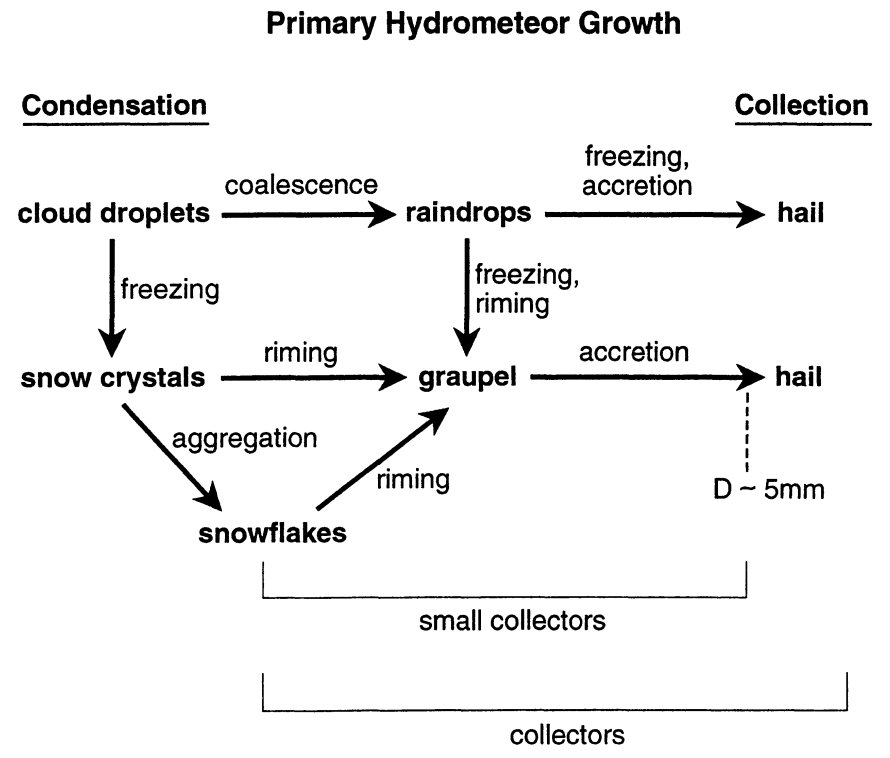
\includegraphics[width=0.7\columnwidth]{figs/growth_knight.png}
		\legend{Fonte: \citeonline{Knight2001}}
	\end{center}
\end{figure}

Dentro da região de fase mista da nuvem, a colisão entre hidrometeoros contribui não só para o crescimento mas também para a troca de cargas entre eles através da transferência de massa. Considerando o momento de dipolo permanente da água, que expõe íons negativos na camada quase-líquida das partículas, a colisão entre dois hidrometeoros transfere íons negativos do hidrometeoro com maior camada para o com menor camada, deixando assim o primeiro positivamente carregado e o segundo negativamente carregado \cite{Baker1987, Baker1994b}. Com a atuação da corrente ascendente, a distribuição de hidrometeoros carregados geram centros de cargas bem definidos dentro da nuvem, e é na interface entre centros de cargas opostas que ocorre a quebra de rigidez dielétrica que origina uma descarga elétrica. Assim, esse mecanismo, chamado de carregamento não-indutivo, é fundamental para a eletrificação de tempestades \cite{Saunders2008}.

A espessura da camada quase-líquida de um hidrometeoro na região de fase mista depende do tipo e tamanho do hidrometeoro e também de fatores externos como conteúdo de água líquida e temperatura. A \autoref{takahashi} mostra o resultado obtido por \citeonline{Takahashi1978} através de medidas em laboratório: após a colisão com cristais de gelo, o graupel fica carregado positivamente independentemente do conteúdo de água líquida em temperaturas mais altas que $-10^{\circ}C$; em temperaturas mais baixas, o graupel fica positivamente carregado quando o conteúdo de água líquida é muito alto (acima de $2\:gm^{-3}$) ou muito baixo (abaixo de $0,2\:gm^{-3}$), enquanto que fica negativamente carregado quando o conteúdo de água líquida está entre $0,2\:gm^{-3}$ e $2\:gm^{-3}$. \citeonline{Williams1991} indicam que o regime de crescimento do graupel/granizo também muda com o conteúdo de água líquida e temperatura (linhas pontilhadas da \autoref{takahashi}): o regime de crescimento é molhado quando o conteúdo de água líquida é muito alto e/ou a temperatura é próxima de $0^{\circ}C$, seco por deposição quando o conteúdo de água líquida e/ou a temperatura são muito baixos e seco por sublimação entre as duas porções anteriores. É importante ressaltar que não há um consenso em relação à esses valores, já que outros estudos feitos em laboratório \cite{Jayaratne1983, Pereyra2000, Saunders2006} não encontraram os mesmos resultados. Os fatores externos descritos aqui são altamente influenciados pela intensidade da corrente ascendente, já que correntes ascendentes mais intensas promovem maior transporte de água líquida para a região de fase mista da nuvem. 

\begin{figure}[hp]
	\begin{center}
		\caption{Carga adquirida pelo graupel/granizo após a colisão com cristais de gelo em função do conteúdo de água líquida e temperatura. As linhas pontilhadas delimitam os regimes de crescimento molhado (porção superior), crescimento seco por sublimação (porção central) e crescimento seco por deposição (porção inferior)} 
		\label{takahashi}
		%		\setcaptionmargin{1cm}
		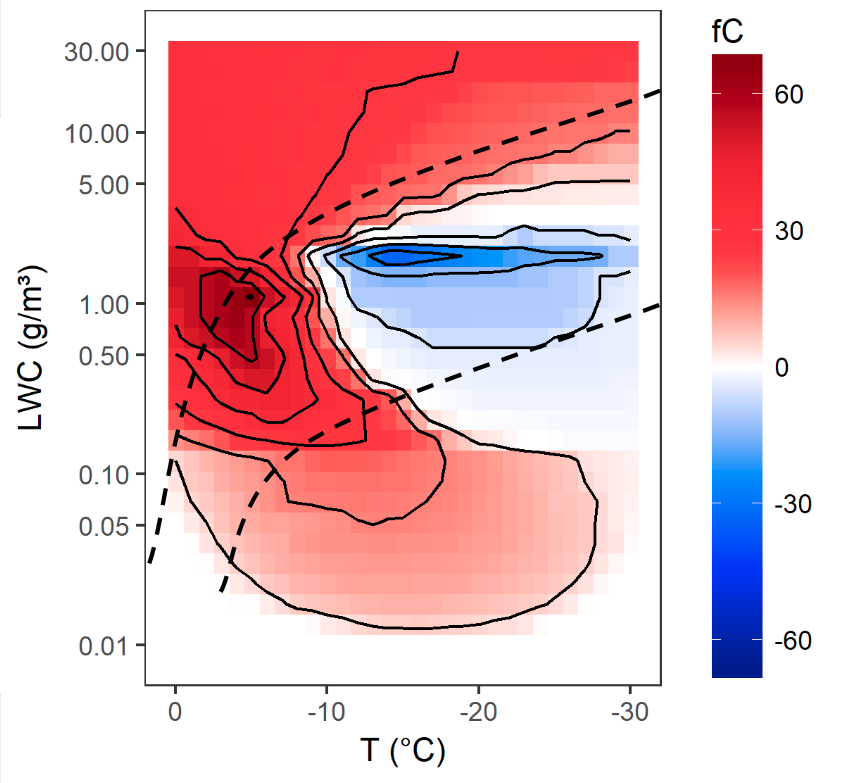
\includegraphics[width=0.6\columnwidth]{figs/takahashi_williams_notitle.png}
		\legend{Fonte: Adaptado de \citeonline{Takahashi1978} e \citeonline{Williams1991}}
	\end{center}
\end{figure}

Simultaneamente à troca de cargas entre graupel/granizo e cristais de gelo, a corrente ascendente transporta e concentra esses hidrometeoros de acordo com a velocidade terminal de cada um: graupel e granizo tendem a entrar em equilíbrio com a corrente ascendente ou descer para fora da região de fase mista, enquanto que os cristais de gelo são transportados para a porção superior ou acima da região de fase mista. Assim, centros de cargas elétricas são formados dentro da nuvem, e a distribuição desses centros depende da complexidade da cinemática da nuvem. Uma descrição simplificada de uma estrutura de cargas na forma de um dipolo foi feita por \citeonline{Wilson1921}, \citeonline{Simpson1937} e \citeonline{Simpson1941}, mas \citeonline{Williams1989} consolidou a estrutura de cargas tripolar como sendo a mais comumente encontrada em tempestades ao revisar diversos experimentos em laboratório e \textit{in-situ}. Essa hipótese considera que o regime de crescimento preferencial do graupel/granizo é seco por deposição, o que significa que eles ficam negativamente carregados; com a atuação da corrente ascendente, um centro de cargas negativas principal é formado na região de fase mista, com dois centros de cargas positivas acima (com cristais de gelo) e abaixo (com hidrometeoros em tamanhos precipitáveis) dessa região, produzindo mais raios nuvem-solo (\textit{cloud-to-ground}, CG) de polaridade negativa (Figura\autoref{tripolar_normal}). Porém, diversos estudos \textit{in-situ}  \cite{Macgorman1994, Carey1995a, Lyons1998, Carey2003e, Carey2007, Pineda2016} mostram que tempestades severas produzem muito mais raios CG de polaridade positiva; dentre as hipóteses que procuram explicar esse fenômeno está a estrutura de tripolo invertido (Figura\autoref{tripolar_oposto}): a corrente ascendente mais intensa aumenta o conteúdo de água líquida na região de fase mista, promovendo o crescimento molhado e carregamento positivo do graupel/granizo; assim, a estrutura simplificada é formada por um centro de cargas positivas na região de fase mista e dois centros de cargas negativas acima e abaixo dessa região, gerando maior quantidade de raios CG positivos. Além disso, tempestades severas também podem promover a formação de granizos gigantes através de ciclos de movimentos descendentes e ascendentes no flanco direito do núcleo de corrente ascendente \cite{Knight1970, Knight2001c, Knight2005} e apresentar picos de atividade elétrica antes da ocorrência de tempo severo (\textit{lightning jump}, salto de raios) \cite{Goodman1988, Williams1999, Schultz2009a, Gatlin2010, Schultz2011}.

\begin{figure}[hp]
	\begin{center}
		\caption{Esquema simplificado de distribuição tripolar de cargas sob ação de uma corrente ascendente em uma tempestade não-severa (a) e uma severa (b)} 
		\label{esquema_tripolar}
		\subfloat[]{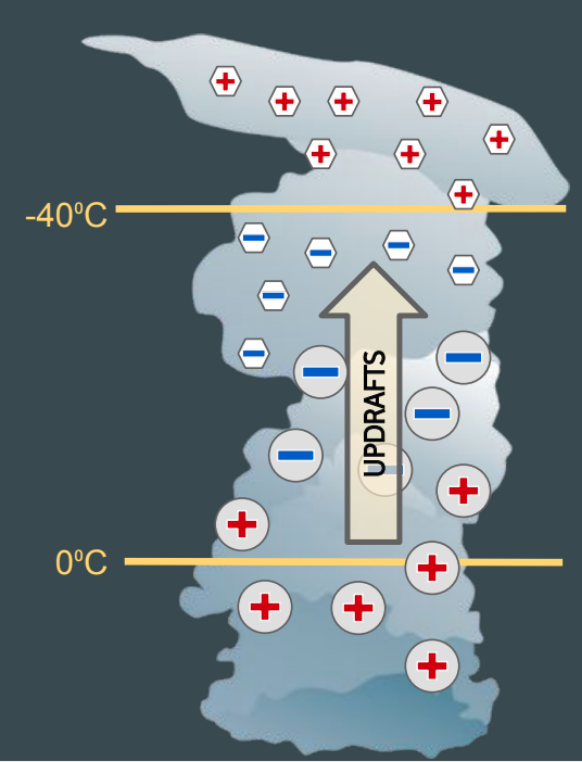
\includegraphics[width=0.35\columnwidth]{figs/tripole_normal.png}
			\label{tripolar_normal}}
		\subfloat[]{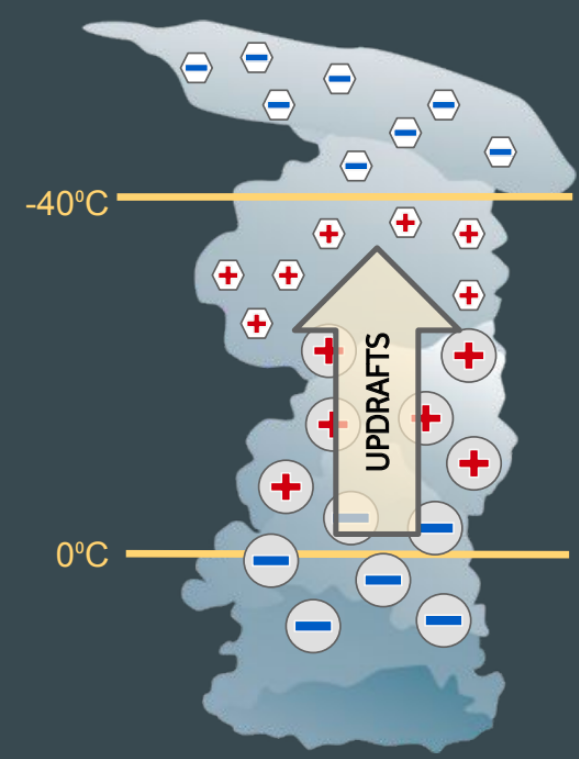
\includegraphics[width=0.35\columnwidth]{figs/tripole_opposite.png}
			\label{tripolar_oposto}} \\
		\legend{Fonte: Produzido pela autora.}
	\end{center}
\end{figure}

\section{Definindo a Intensidade das Tempestades de Granizo}

Tempestades de granizo são definidas como nuvens com produção de granizo de tamanho suficiente para 

\section{Tempestades de Granizo na América do Sul}

Diferentemente de tempestades em latitudes médias, tempestades tropicais raramente são intensas o suficiente para gerar queda de granizo ou graupel no solo, com exceção da África Central \cite{Court1982, Hand2011, Cecil2012a}. Como mostrado na \autoref{sinotica_barnes}, a porção central e norte da América do Sul não apresenta condições sinóticas que favoreçam a formação de convecção organizada e sistemas convectivos de mesoescala (por ser um ambiente barotrópico, com baixos gradientes de temperatura), apenas tempestades isoladas principalmente durante o verão (Figura\autoref{sinotica_jan}); essas tempestades costumam ter pouco tempo de vida e correntes ascendentes insuficientes para transportar grandes quantidades de água líquida para a região de fase mista e promover o crescimento de granizo. Já mais ao sul, tempestades de granizo destrutivas têm sido relatadas na Argentina subtropical e na região sul do Brasil \cite{Court1982, Martins2017}; satélite, modelagem e climatologias mostram que essa área pode chegar a $\ang{15}S$ de latitude \cite{Hand2011, Cecil2012a, Albrecht2016}.

\begin{figure}[htb]
	\begin{center}
		\caption{Esquema com as características de escala planetária e sinótica primárias encontradas na superfície no Atlântico Tropical em janeiro (a) e julho (b)} 
		\label{sinotica_barnes}
		\subfloat[]{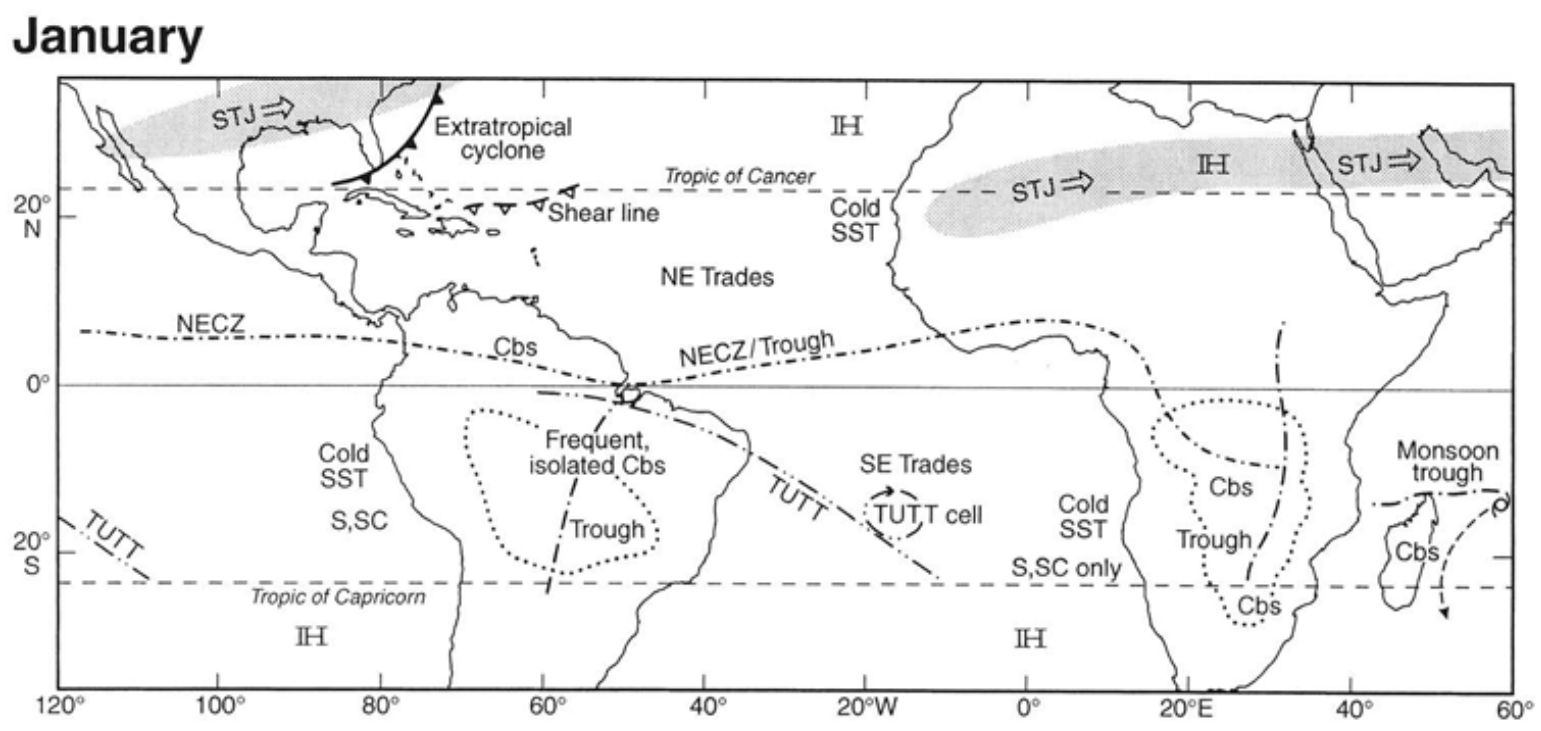
\includegraphics[width=0.8\columnwidth]{figs/barnes_synoptic_jan.png}
			\label{sinotica_jan}} \\
		\subfloat[]{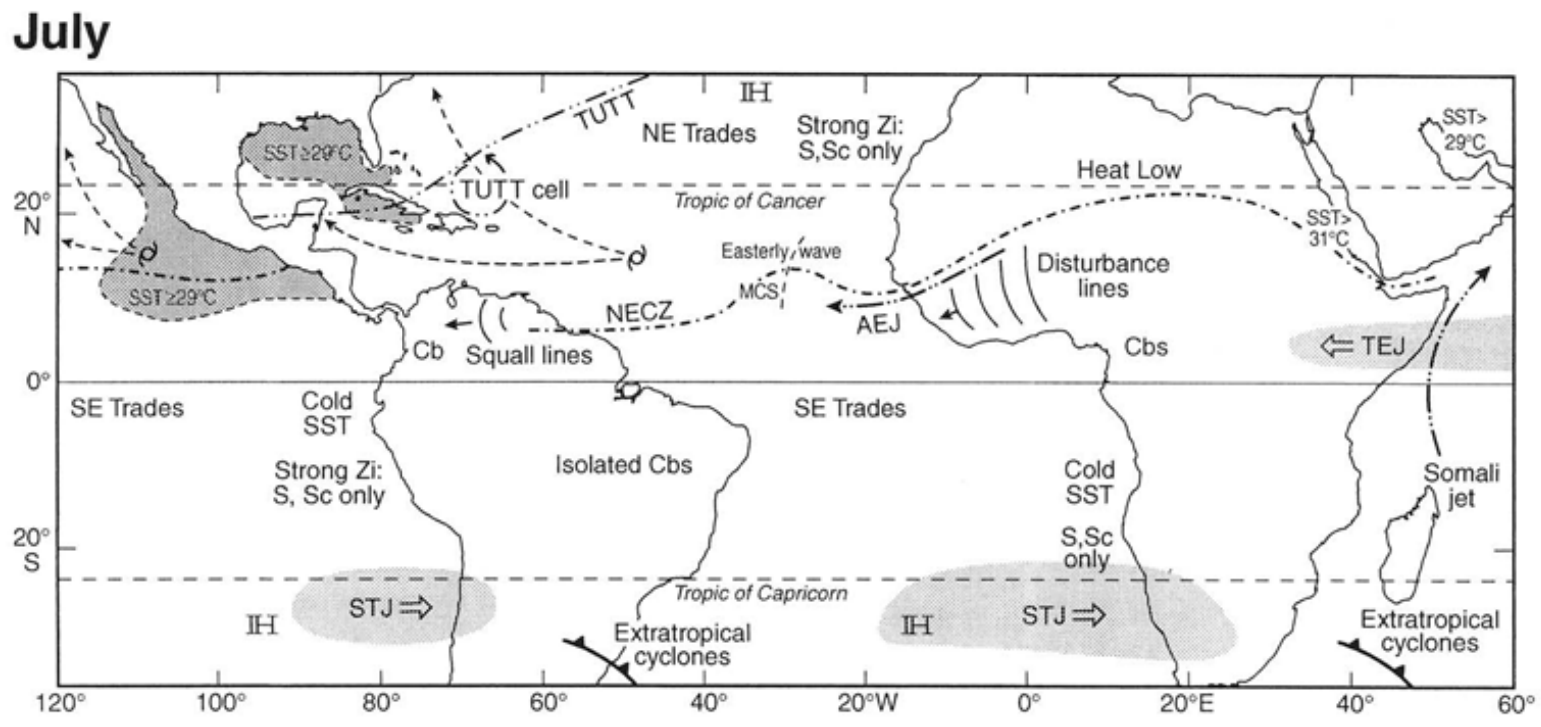
\includegraphics[width=0.8\columnwidth]{figs/barnes_synoptic_jul.png}
			\label{sinotica_jul}} \\
		\legend{Fonte: \citeonline{Barnes2001}}
	\end{center}
\end{figure}

A \autoref{climatologia_granizo} mostra uma climatologia de tempestades de granizo severas (ou seja, com queda de granizos grandes ou gigantes) no sudeste da América do Sul usando uma série temporal de 8 anos de dados do sensor passivo em microondas AMSR-E (\textit{Advanced Microwave Scanning Radiometer for Earth Observing System}, Radiômetro Avançado de Escaneamento em Microondas para o Sistema de Observação Terrestre) a bordo do satélite de órbita sincronizada com o Sol \textit{Aqua}. O pico de frequência de tempestades de granizo está centrado no norte da Argentina, se estendendo ao Paraguai, Uruguai e partes de Brasil e Bolívia \cite{Cecil2012a}. \citeonline{Barnes2001} (em sua Figura 10.31) mostra que o ciclo anual de eventos de granizo no Brasil (entre 18 e $\ang{22}S$) é sazonal, com maior frequência na primavera e verão. \citeonline{Sperling2018} também mostra maior frequência de granizo durante a primavera considerando eventos no sul do Brasil, que são produzidos por tempestades isoladas de grande extensão vertical antes de se juntarem a sistemas convectivos de mesoescala formados ao longo do jato sul-americano de baixos níveis em situações pré-frontais. Essas tempestades são formadas por pequenas células convectivas explosivas que rapidamente (abaixo de 30 minutos) desenvolvem uma região de fase mista com refletividade acima de $50\:dBZ$ até $18\:km$ de altura; entre 10 e 20 minutos depois do crescimento explosivo das células e aumento da massa de gelo, há um distinto salto na taxa de raios totais, produzindo granizo com mais de $6\:cm$ de diâmetro observado no solo. No sudeste do Brasil, incluindo a região de estudo desta dissertação, a frequência e tamanho do granizo são menores que no sul do Brasil, mas também produzidos por pequenas células convectivas em situações pré-frontais \cite{Puig2017}.

\begin{figure}[htb]
	\begin{center}
		\caption{Climatologia anual de granizo a partir do sensor AMSR-E para o sudeste da América do Sul. Os contornos em cinza indicam a elevação, com intervalos de $1\:km$} 
		\label{climatologia_granizo}
		%		\setcaptionmargin{1cm}
		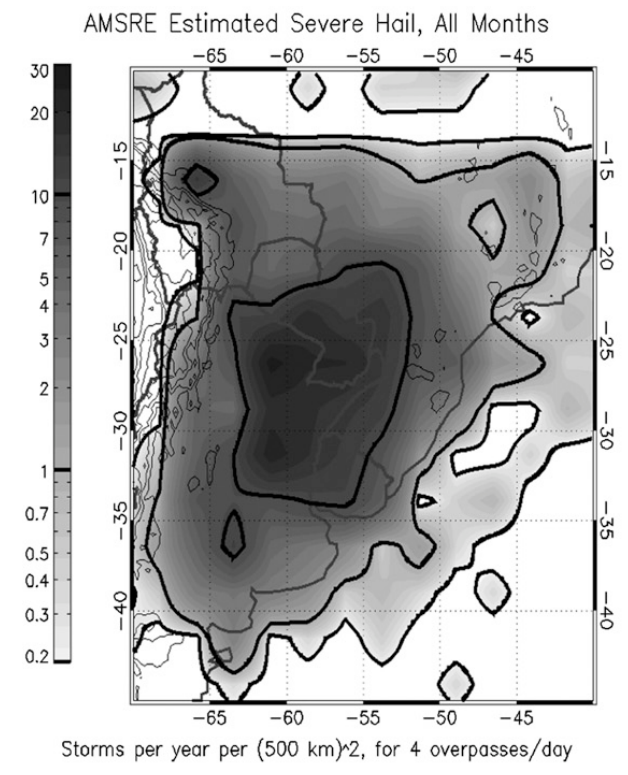
\includegraphics[width=0.5\columnwidth]{figs/cecil_severehail.png}
		\legend{Fonte: \citeonline{Cecil2012a}}
	\end{center}
\end{figure}

\section{Usando Radares Meteorológicos para Estudar a Cinemática das Tempestades}

Radares Doppler possuem a capacidade de medir a velocidade dos alvos que estão em seu volume observado, gerando essa importante informação sobre as nuvens com alta resolução espacial. A partir da velocidade da precipitação desses alvos, é possível derivar não só o deslocamento da nuvem em si como também o escoamento dentro da nuvem, inferindo assim as propriedades cinemáticas da nuvem e sua importância para o ciclo de vida. É possível extrair informações relacionadas ao campo de vento a partir da recuperação das componentes do vento com um  (display de velocidade-azimute (VAD, \textit{velocity-azimuth display}); para mais informações, ver seção 11.5 de \citeonline{Rauber2018}) ou mais radares (Dual ou Multi-Doppler; gera um campo tridimensional do vento). Para tempestades de granizo, por exemplo, \citeonline{morgan1986thunderstorm} afirmam que técnicas Dual ou Multi-Doppler oferecem a descrição mais realista do ambiente relacionado ao granizo, pois permite observar efeitos de advecção com alto grau de detalhamento.

Desde a primeira formulação do método de recuperação de vento tridimensional \cite{Armijo1969}, diversos trabalhos usaram este método para entender a cinemática de tempestades. Estudos pioneiros descrevem a estrutura de tempestades severas \cite{Brandes1977, Ray1980}, frentes de rajada \cite{Weaver1982}, tempestades não-severas usando Multi-Doppler \cite{Ray1978} e microexplosões \cite{Wilson1984} nos Estados Unidos, além do estudo de uma linha de instabilidade tropical no oeste da África \cite{Chong1987}. O desenvolvimento de métodos e ferramentas mais sofisticadas permitiu estudos detalhados de tempestades que causaram grandes volumes de precipitação \cite{Petersen1999a, Calhoun2013} e supercélulas \cite{Potvin2012a, Potvin2012b}, incluindo um caso com sucessivas tornadogêneses \cite{Wurman2007}; \citeonline{Hubbert1998a} usou o método Dual-Doppler para auxiliar na identificação dos processos microfísicos associados à assinaturas nas variáveis polarimétricas em um caso com queda de granizos gigantes. Outros estudos buscaram estudar a estrutura de diversas tempestades para descrever as principais diferenças na cinemática convectiva entre tempestades severas e não-severas \cite{Lang2002, Deierling2008}. No Brasil, o experimento TRMM-LBA (\textit{Tropical Rainfall Measuring Mission Large Scale Biosphere–Atmosphere Experiment in Amazonia}, Experimento de Larga Escala Biosfera-Atmosfera na Amazônia da Missão de Medidas de Precipitação Tropical) gerou diversos estudos da cinemática de tempestades tropicais na Amazônia durante o período chuvoso \cite{Rutledge2000, Cifelli2002b, Cifelli2004a}, mostrando que as tempestades que se desenvolvem em um escoamento de leste em baixos níveis apresentam extensão vertical maior e correntes ascendentes mais intensas comparando com as que se desenvolvem em um escoamento de oeste.

A base teórica do método de recuperação de vento tridimensional consiste em determinar 4 componentes da velocidade do vento em coordenadas cartesianas: $u$, $v$, $w$ e $w_t$, onde as três primeiras são as componentes da velocidade nas coordenadas $x$, $y$ e $z$ e $w_t$ é a velocidade terminal da precipitação \cite{Rinehart1997}. Dois radares Doppler vendo a mesma tempestade de ângulos diferentes fornecem duas medidas distintas de velocidade radial ($v_{r_1}$ e $v_{r_2}$), como mostra a \autoref{doviak_sistema}, e $w_t$ pode ser estimada em função da refletividade (usando uma distribuição de Marshall-Palmer, por exemplo). Assim, $u$ e $v$ podem ser descritos como:

\begin{figure}[htb]
	\begin{center}
		\caption{Sistema de coordenadas cilíndricas usado para análise Dual-Doppler de dados de radar. Os radares estão localizados nos pontos 1 e 2 e $a_r$, $a_s$ e $a_\alpha$ são as normais unitárias definindo a direção das três componentes ortogonais da velocidade. O eixo cilíndrico está ao longo da linha conectando os radares (separados por uma distância $2d$) e $r$ é a distância do eixo ao dado pontual} 
		\label{doviak_sistema}
		%		\setcaptionmargin{1cm}
		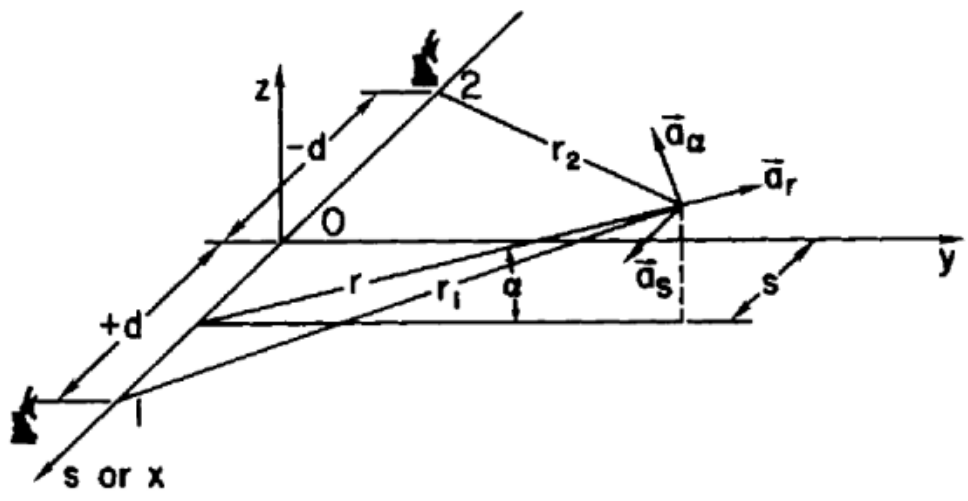
\includegraphics[width=0.8\columnwidth]{figs/system_doviak.png}
		\legend{Fonte: \citeonline{Doviak1993}}
	\end{center}
\end{figure}

\begin{equation}
u=\frac{1}{\sin{(\theta_1 - \theta_2)}}\left(\frac{v_{r_1}\cos{\theta_2}}{\sin{\alpha_1}}-\frac{v_{r_2}\cos{\theta_2}}{\sin{\alpha_2}}\right)
\end{equation}

\begin{equation}
v=\frac{1}{\sin{(\theta_1 - \theta_2)}}\left(\frac{v_{r_2}\cos{\theta_1}}{\sin{\alpha_2}}-\frac{v_{r_1}\cos{\theta_1}}{\sin{\alpha_1}}\right)
\end{equation}

\noindent
onde $\theta_1$ e $\theta_2$ são os ângulos azimutais dos radares $1$ e $2$, respectivamente, e $\alpha_1$ e $\alpha_2$ são os ângulos de elevação dos mesmos.

Para calcular a componente vertical da velocidade, a equação de continuidade de massa é usada, assumindo como condições de contorno que a velocidade na superfície e no topo da tempestade são nulas, ou seja:

\begin{equation} 
\label{continuidade_massa}
\frac{\partial(\rho w)}{\partial z}=-\rho\left(\frac{\partial u}{\partial x} + \frac{\partial v}{\partial y}\right)
\end{equation}

\begin{equation}
w=w_T-w_t
\end{equation}

\noindent
onde $\rho$ é a densidade do ar atmosférico e $w_T$ é a velocidade vertical total. Quando três radares são usados, é possível calcular o campo tridimensional sem usar a \autoref{continuidade_massa}.

Ao combinar radares Doppler para a recuperação do vento, a área de cobertura e erros característicos (altura do feixe e resolução espacial) devem ser considerados \cite{Dolan2007}. Se a distância da linha de base entre os dois radares for longa, a área de cobertura será maior mas a resolução espacial será prejudicada. Além disso, se o ângulo de cruzamento do feixe é pequeno (mais paralelo), as duas medidas serão mais similares e as variâncias dos erros de velocidade nas estimativas Dual-Doppler - $\sigma_u^2$ e $\sigma_v^2$ - serão menores. De acordo com \citeonline{Davies-Jones1979}, $\sigma_u^2$ e $\sigma_v^2$ estão relacionadas com as variâncias dos erros de velocidade Doppler de cada radar, $\sigma_1^2$ e $\sigma_2^2$, da seguinte forma:

\begin{equation}
\frac{\sigma_u^2+ \sigma_v^2}{\sigma_1^2 + \sigma_2^2}=\csc^2{\beta}
\end{equation}

\noindent
onde $\beta$ é o ângulo de cruzamento do feixe entre os dois radares. Para $\beta\:<\:\ang{30}$, $\sigma_u^2$ e $\sigma_v^2$ crescem rapidamente \cite{Doviak1976, Davies-Jones1979, Doviak1993}.

A \autoref{doppler_theory_lobes} mostra teoricamente as áreas aceitáveis para estimativa de velocidade do vento considerando dois valores de $\beta$: $\ang{30}$ e $\ang{45}$. Quanto maior o valor de $\beta$, melhor é a estimativa Dual-Doppler, mas menor será a área de cobertura dessa estimativa.

\begin{figure}[htb]
	\begin{center}
		\caption{Ângulos teóricos de cruzamento do feixe com Dual-Doppler de \ang{45} (melhores dados de vento) e \ang{30} (dados de vento aceitáveis) para um par de radares Doppler} 
		\label{doppler_theory_lobes}
		%		\setcaptionmargin{1cm}
		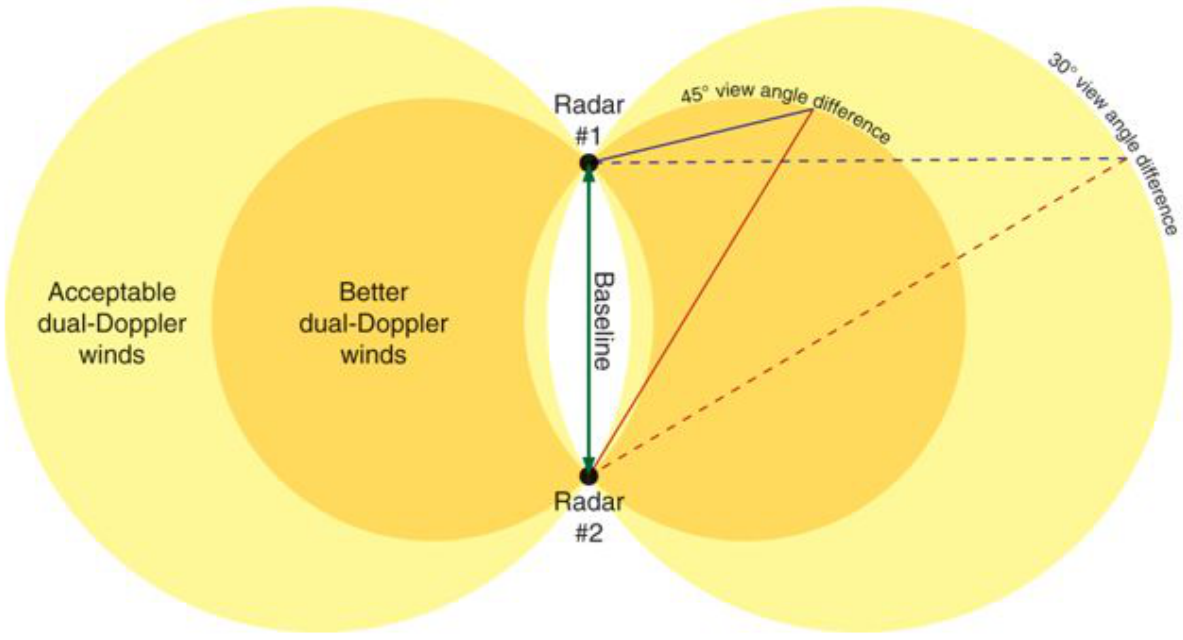
\includegraphics[width=\columnwidth]{figs/lobes_eastin.png}
		\legend{Fonte: Dr. Matthew D. Eastin, UNC.}
	\end{center}
\end{figure}

